\documentclass[__main__.tex]{subfiles}

\begin{document}

\qtitle{О}{03}
Рассмотрите электромагнитные волны в пространстве, свободном от зарядов и токов. Покажите, что вектора $\vec{k}$ (волновой вектор), $\vec{E}$, $\vec{B}$ образуют правую тройку в некоторой инерциальной системе отсчёта. Объясните, почему в любой другой инерциальной системе отсчёта этот факт, будучи сформулированным для преобразованных векторов, будет также иметь место.\\

\begin{definition}
\textit{Волновым вектором} называется
$$
\vec{k}=\frac{\omega}{V}\vec{n},
$$
где $\vec{n}$ -- единичный вектор распространения волны, $V$ - скорость распространения волны.
\end{definition}

\begin{definition}
Процесс распространения электромагнитного поля в пространстве называется \textit{электромагнитной волной}.
\end{definition}

Если в точке $A$ создано электрическое поле $E_1$, убывающее со временем, это соответствует появлению тока смещения, направленного к точке А, и возникновению перпендикулярно к току вихревого магнитного поля $B_1$. Магнитное поле убывает вследствие отсутствия поддерживающих его токов.

Убывающее магнитное поле порождает вихревое электрическое поле $E_2$ в пространстве в <<контуре>> $l$. Направление $E_2$ подчиняется \textit{правилу Ленца} (Индукционный ток всегда имеет такое направление, что он ослабляет действие причины, возбуждающей этот ток). Поле $E_2$ убывает, порождается магнитное поле $B_2$ и т.д. Электромагнитная волна распространяется со скоростью $V$ вдоль оси $Oz$ (см. Рис. 79). Таким образом:

\begin{enumerate}
\item
электромагнитная волна поперечна, колебания $\vec{E}$ и $\vec{B}$ проходят перпендикулярно направлению распространения волны (см. Рис. 80);
\item
электрическое и магнитное поля в бегущей волне изменяются в одной фазе;
\item
$\vec{E}$, $\vec{B}$ и $\vec{V}$ (а вместе с ним и $\vec{k}$) в бегущей электромагнитной волне образуют так называемую правую тройку векторов.
\end{enumerate}

\begin{figure}[h]
\begin{minipage}{.6\linewidth}
    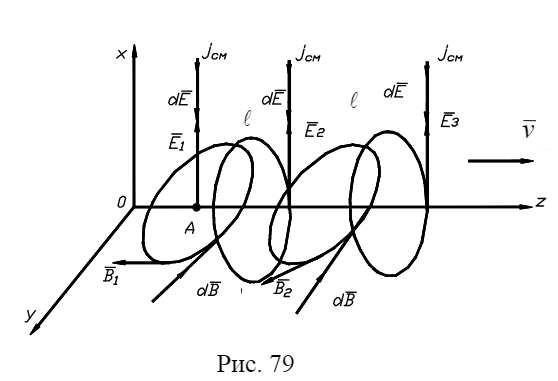
\includegraphics[width=1\linewidth]{e02_1.png}
\end{minipage}
\hfill
\begin{minipage}{.4\linewidth}
    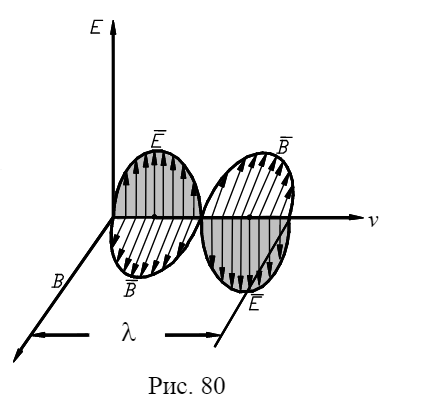
\includegraphics[width=1\linewidth]{e02_2.png}
\end{minipage}
\end{figure}

\end{document}